\chapter{Teoría de Sistemas Lineales}



\section{Matriz de transición de Estados}
Sea un sistema LTI autónomo (es decir, sin entrada u)
\begin{align*}
    \tend{\dot{x}}(t)=\tenq{A}\tend{x}(t), \quad \tend{x}(0)=\tend{x_0}
\end{align*}
La solución $\tend{x}(t)$ se puede obtener utilizando transformación de Laplace:\\
\par \underline{Definición}: $\mathcal{L}\{\tend{x}(t)\}=\tend{X}(s)$\\
\par \underline{Definición}: $\mathcal{L}\{\tend{\dot{x}}(t)\}=s\tend{X}(s)-\tend{x_0}$\\
\par Reemplazando:
\begin{align*}
    \Longrightarrow s\tend{X}-\tend{x_0} &= \tenq{A}\tend{X}\\
    \Longrightarrow (s\tenq{I}-\tenq{A})\tend{X} &=\tend{x_0}\\
    \Longrightarrow \tend{X}(s) &= (s\tenq{I}-\tenq{A})^{-1}\tend{x_0}\\
    \Longrightarrow \tend{x}(t) &= e^{\tenq{A}t}\tend{x_0}\\
    \Longrightarrow \tend{x}(t) &= \tenq{\phi}(t)\tend{x_0}
\end{align*}
Donde $\tenq{\phi}(t)=e^{\tenq{A}t}$ es la \textcolor{red}{matriz de transición de estados del sistema}. \\
\par \underline{Aparte}: Expansión e series de Taylor.\\
Sea f(t) es continua y suave, entonces la expansión de Taylor respecto a $t=\alpha$
$$f(t)=f(\alpha)+\frac{\dot{f}(\alpha)}{1!}(t-\alpha)+\frac{\ddot{f}(\alpha)}{2!}(t-\alpha)^2+... $$
Podemos utilizar esto para escribir una expansión de la función escalar $f(t)=e^{at}$, para $\alpha=0$.
$$e^{at}=1+at+\frac{1}{2!}a^2t^2+\frac{1}{3!}a^3t^3+... $$

\par Se puede demostrar que la expansión de Taylor de $\tenq{\phi}(t)$:
\begin{align*}
    \tenq{\phi}(t)=e^{\tenq{A}t}=\tenq{I}+\tenq{A}t+\frac{1}{2!}\tenq{A}^2t^2+\frac{1}{3!}\tenq{A}^3t^3+...
\end{align*}

\underline{Nota}: $\tenq{\phi}(t)$ satisface la ecuación de estado:
\begin{align*}
    \Longrightarrow \tend{x}(t) &= \tenq{\phi}(t)\tend{x_0}\\
    &= \left[\tenq{I}+\tenq{A}t+\frac{1}{2!}\tenq{A}^2t^2+...\right]\tend{x_0}\\
    \Longrightarrow \tend{\dot{x}}(t) &= \left[\tenq{A}+\frac{2}{2!}\tenq{A}^2t+...\right]\tend{x_0}\\
    &= \tenq{A}\left[\tenq{I}+\tenq{A}t+\frac{1}{2!}\tenq{A}^2t^2+...\right]\tend{x_0}\\
    \Longrightarrow \tend{\dot{x}}(t) &= \tenq{A}\tenq{\phi}(t)\tend{x_0}=\tenq{A}\tend{x_t} \quad \text{Ecuación de Estado}
\end{align*}

Si tenemos un sistema LTI no autónomo:
\begin{align*}
    \tend{\dot{x}}(t) &= \tenq{A}\tend{x}(t)+\tenq{B}\tend{u}(t)\\
    \Longrightarrow s\tend{X}-\tend{x_0} &= \tenq{A}\tend{X}+\tenq{B}\tend{U}\\
    \Longrightarrow (s\tenq{I}-\tenq{A})\tend{X} &= \tend{x_0}+\tenq{B}\tend{U}\\
    \Longrightarrow \tend{X}(s) &= (s\tenq{I}-\tenq{A})^{-1} \tend{x_0}+(s\tenq{I}-\tenq{A})^{-1} \tenq{B}]tend{U}(s)\\
    \Longrightarrow \tend{x}(t) &= \tenq{\phi}(t)\tend{x_0}+\left[ \tenq{\phi}(t)\tenq{B} \right] \ast u(t)\\
    \tend{x}(t) &= \tenq{\phi}(t)\tend{x_0}+\int_0^t\tenq{\phi}(t-\tau)\tenq{B}\tend{U}(\tau)d\tau
\end{align*}

Solución $\tend{x}(t)$ del sistema LTI no-autónomo.\\
\par Sobre las propiedades de $\tenq{A}$, del problema de valores propios:
$$\tenq{A}\tend{v}=\lambda\tend{v}$$
donde $\tend{v}$ y $\lambda$ son el vector y valor propio asociado.
\begin{align*}
    \Longrightarrow \tenq{\phi}(t)\tend{v} &= \left[\tenq{I}+\tenq{A}t+\frac{1}{2!}\tenq{A}^2t^2+...\right]\tend{v}\\
    &= \tend{v}+\tenq{A}\tend{v}t+\frac{1}{2!}\tenq{A}^2\tend{v}t^2+... \\
    &= \tend{v}+\lambda\tend{v}t+\frac{1}{2!}\lambda^2\tend{v}t^2+... \\
    &= \left[ 1+\lambda t+\frac{\lambda^2}{2!}+\frac{\lambda^3}{3!}t^3\right]\tend{v}
\end{align*}
Si $\tend{x_0}=\tend{v}$, entonces $\tend{x}(t)=\tenq{\phi}(t)\tend{v}$\\
\par Pregunta: ¿Es $\phi(t)$ una serie infinita?\\
$$\lim_{t \to \infty} \phi(t)<\infty $$ sí y solo si $\text{Re}(\lambda)<0$. 
Entonces el sistema LTI es estable!\\

\par \underline{Definición}: Una matriz $\tenq{A}$ se dice que es \textcolor{red}{Hurwitz} ssi los valores propios de $\tenq{A}$ tienen una parte real estrictamente negativa.


\section{Plano de Fase}
Representación gráfica de las trayectorias de un sistema dinámico autónomo en el plano.
\begin{figure}[H]
\centering
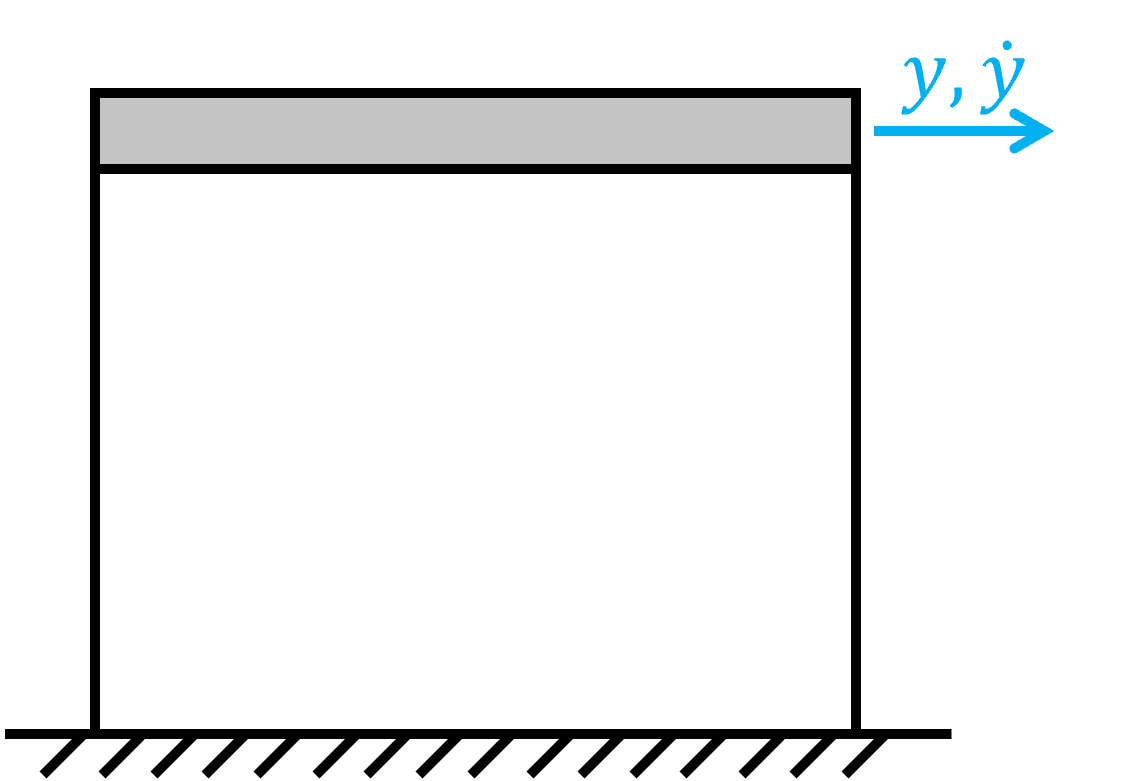
\includegraphics[scale=0.7]{Figuras/leccion11.png}
\end{figure}
\begin{align*}
    \Longrightarrow \tend{\dot{x}}(t) =\tend{f}(\tend{x},t)=\tenq{A}\tend{x}(t)
\end{align*}
donde 
$\tend{x}=\begin{bmatrix}\tend{y}\\ \tend{\dot{y}}\end{bmatrix}$, con condiciones iniciales $y_0$, $\dot{y}_0$.
\begin{figure}[H]
\centering
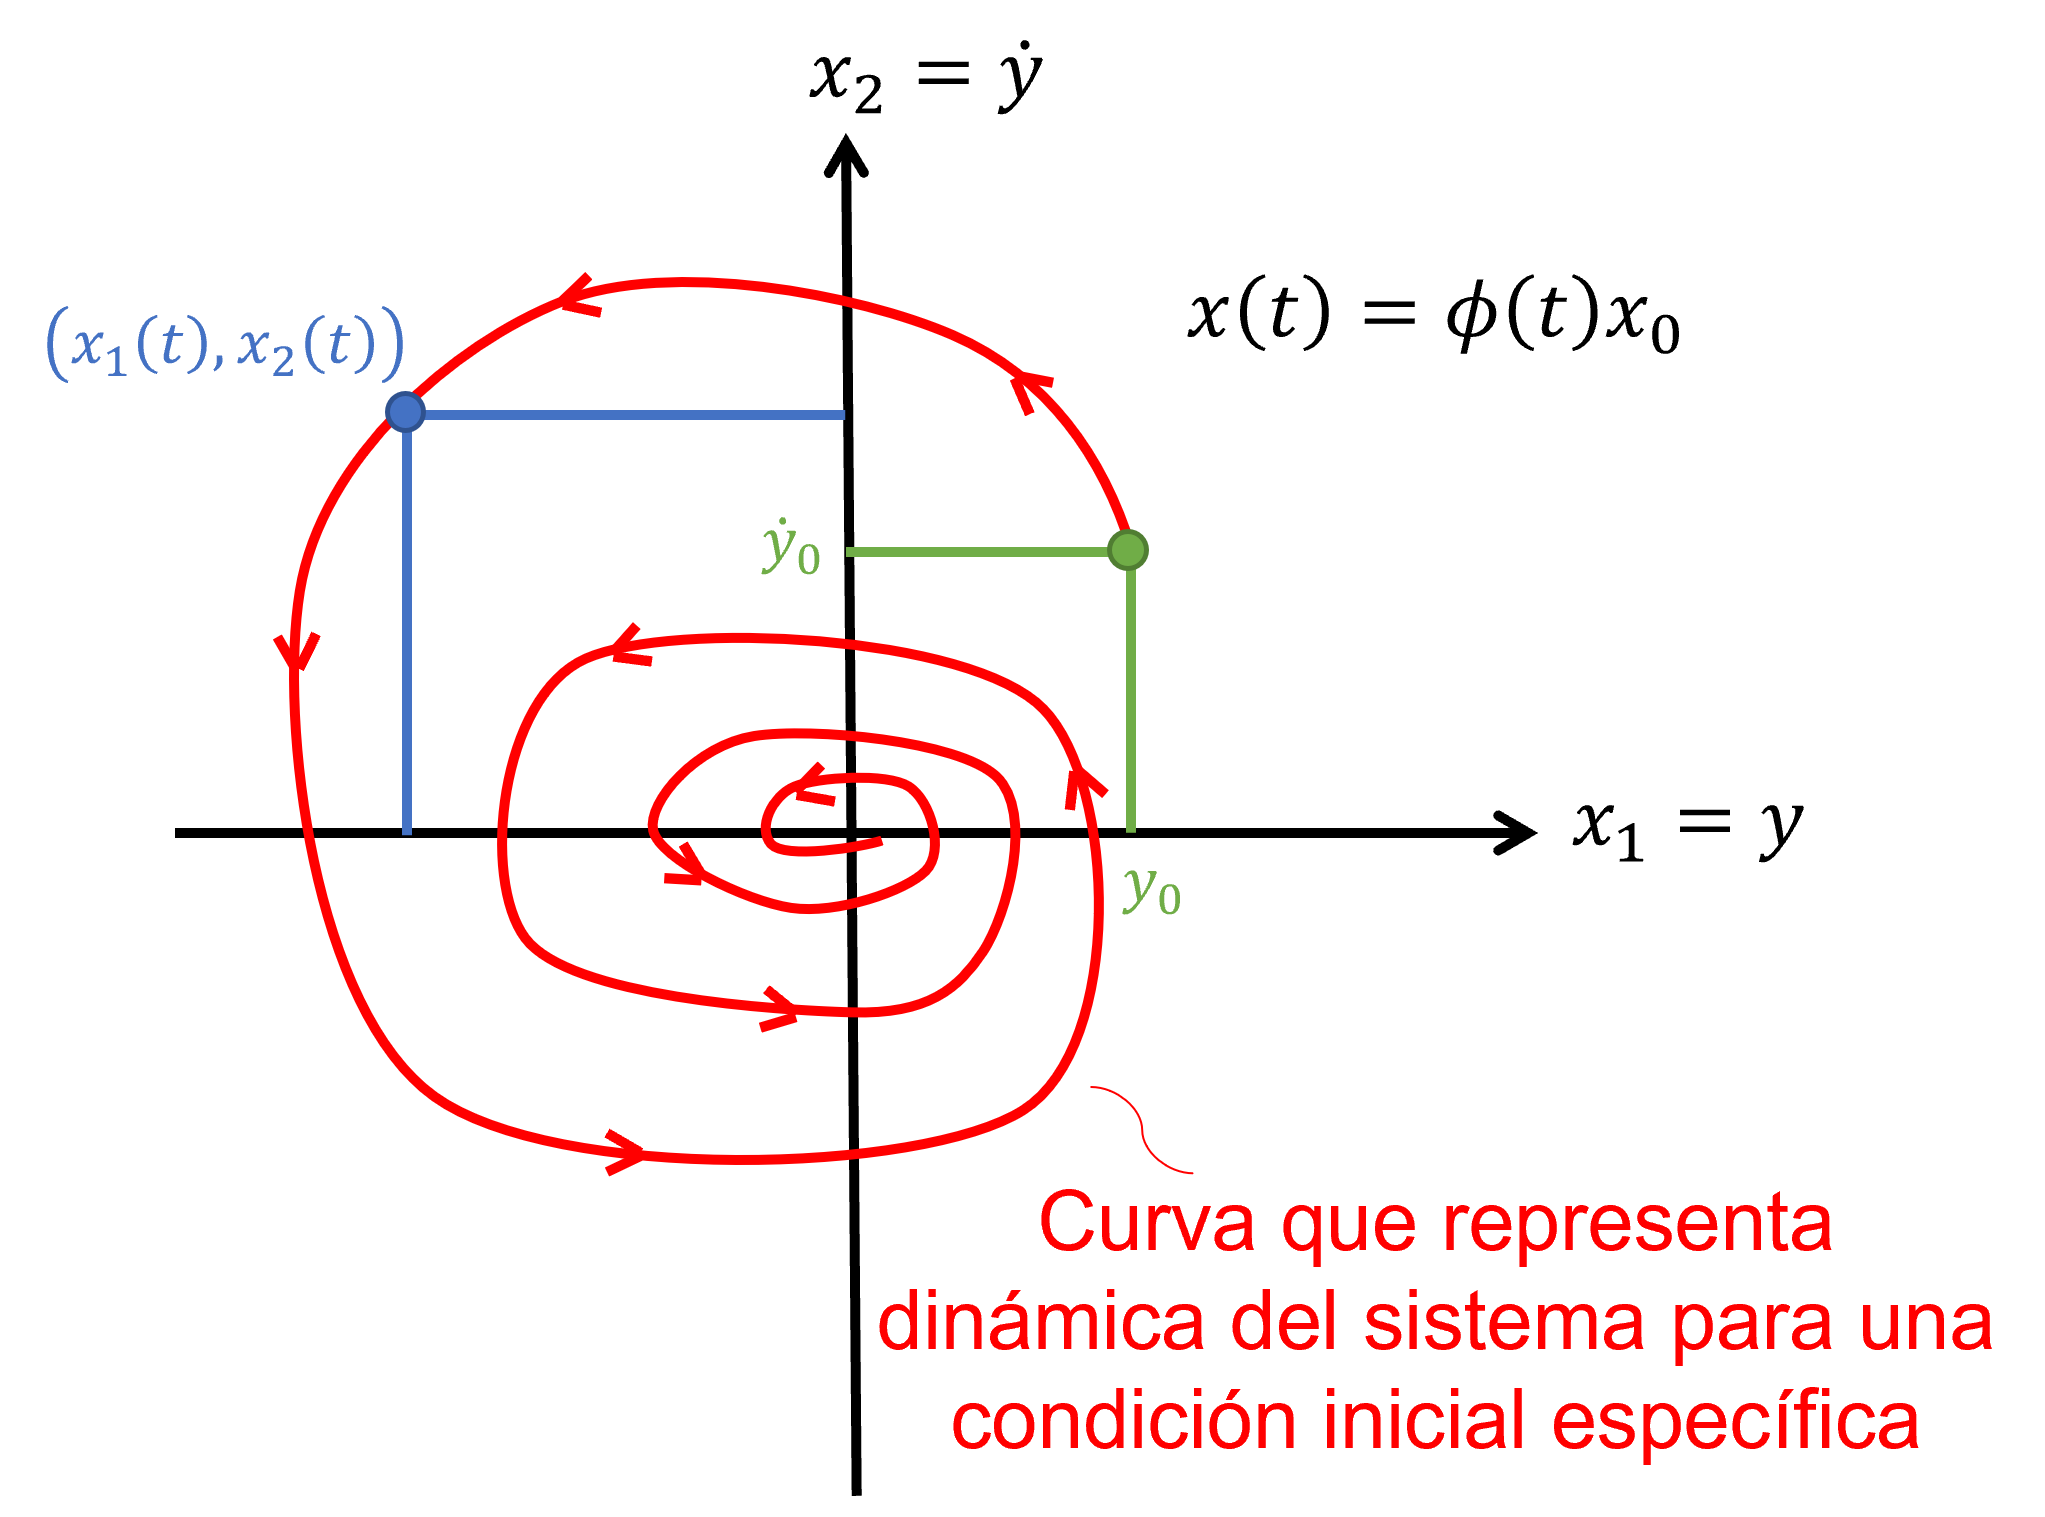
\includegraphics[scale=0.7]{Figuras/plano_de_fase.png}
\end{figure}
\begin{figure}[H]
\centering
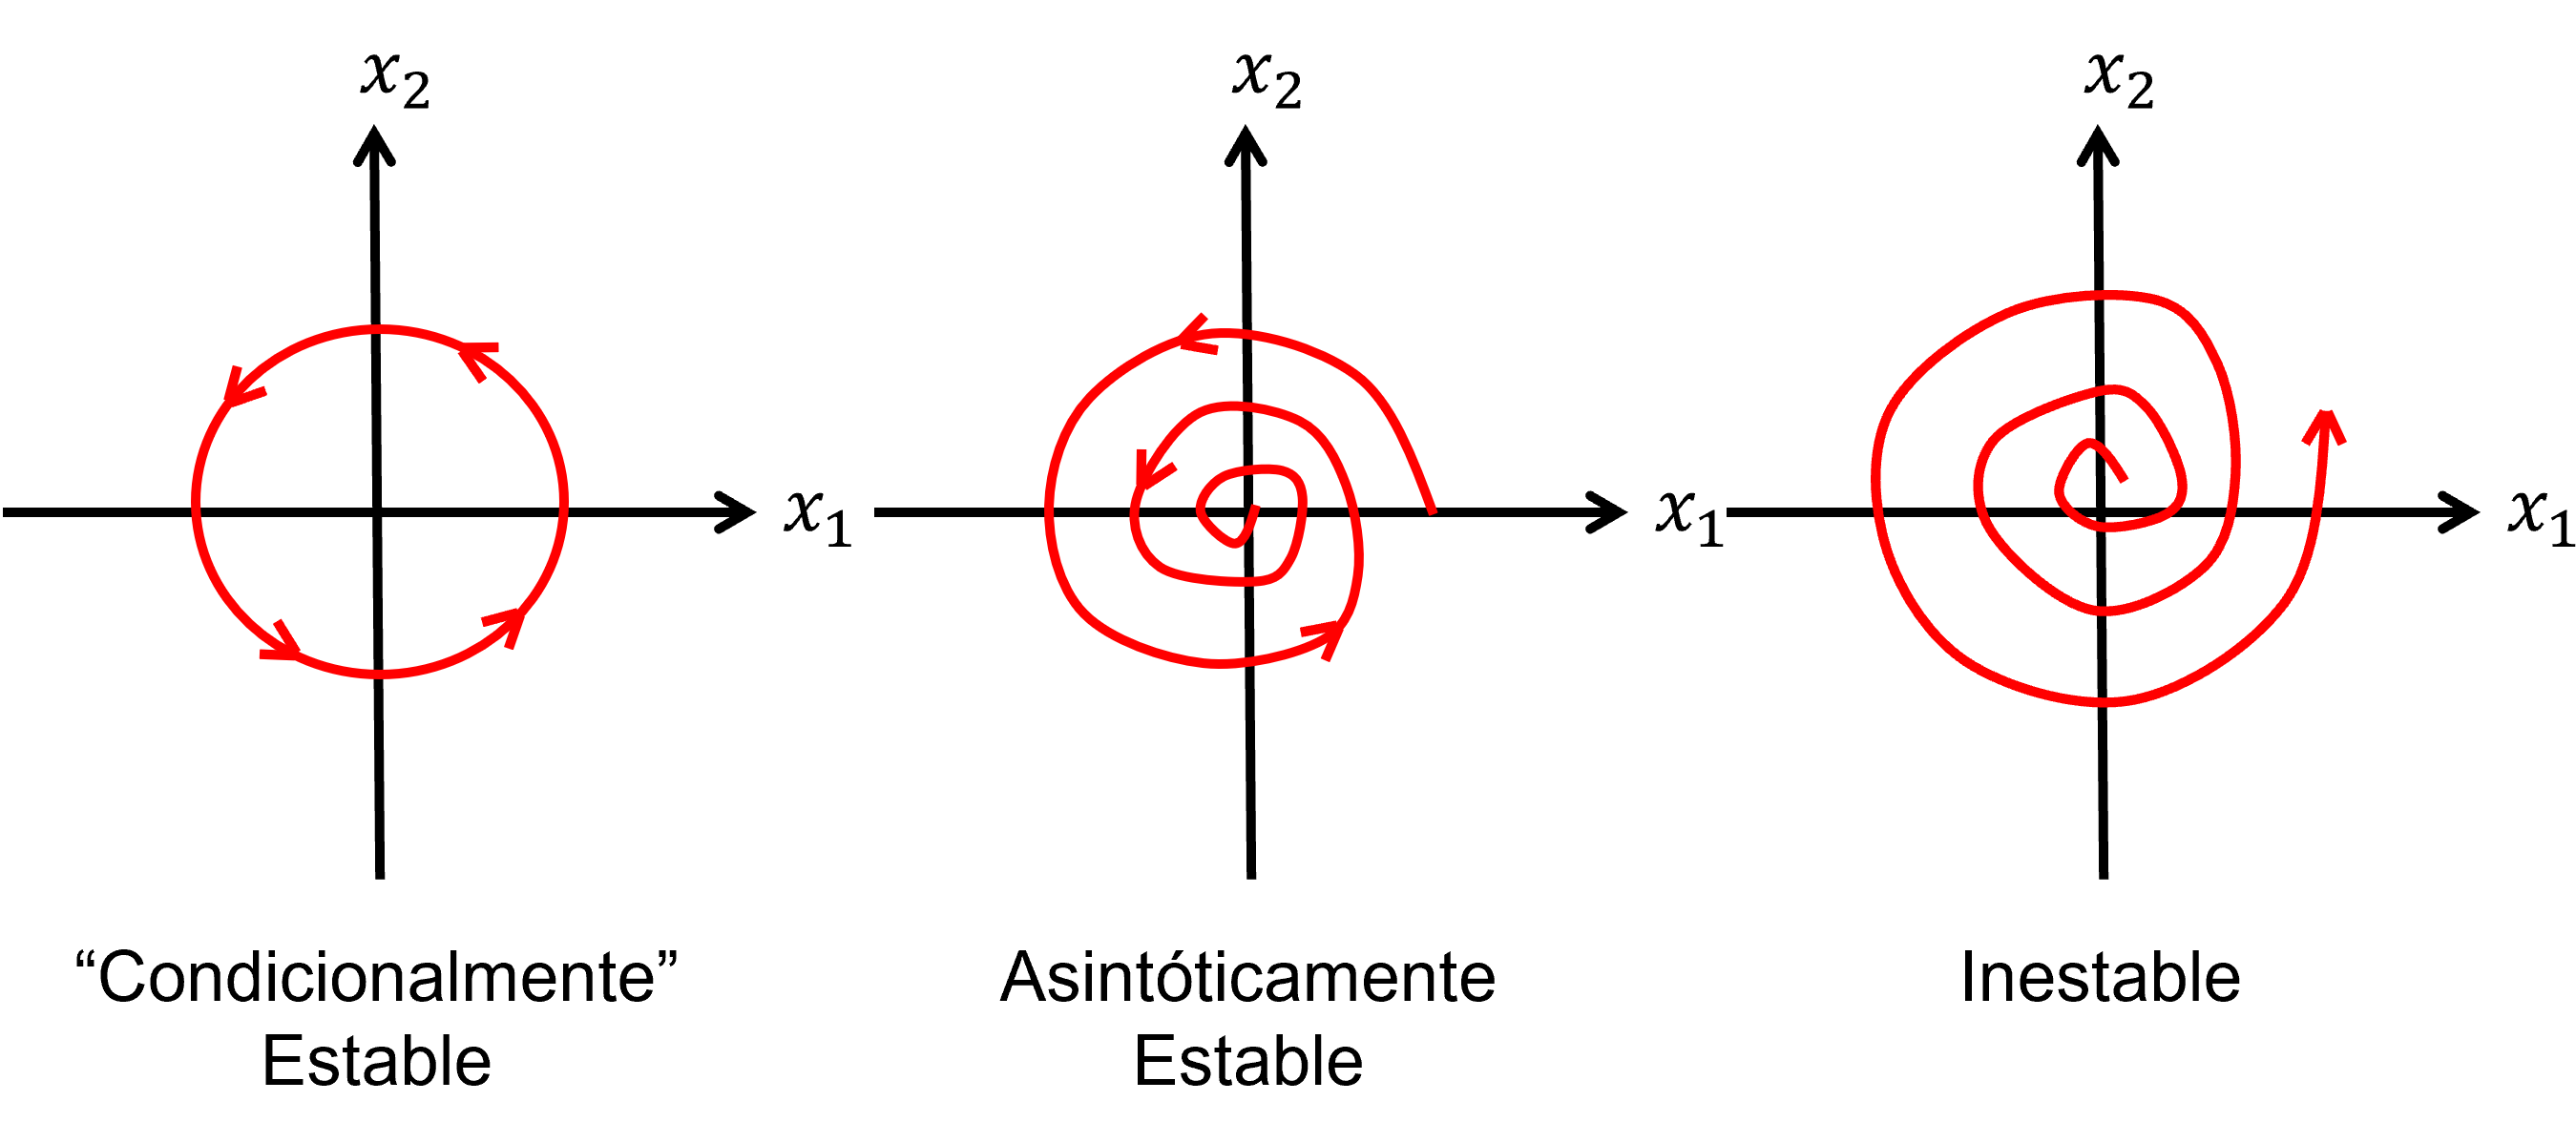
\includegraphics[scale=0.7]{Figuras/plano_de_fase.png_2.png}
\end{figure}

\section{Equilibrio}
Sea el sistema dinámico LTI:
$$\tend{\dot{x}}=\tenq{A}\tend{x}+\tenq{B}\tend{u} $$

\underline{Definición}: El equilibrio del sistema está dado por:
$$ \tend{\dot{x}}=\tend{0} \Longrightarrow \tend{x} \text{ no cambia con el tiempo}$$
Entonces:
\begin{align*}
    \Longrightarrow \tend{0}=\tenq{A}]\tend{x_e}+\tenq{B}\tend{u_e} \\
\end{align*}
donde $\tend{x_e}$ s el vector de estado en equilibrio y $\tend{u_e}$ es el vector de entrada en el equilibrio = constante.
\begin{align*}
    \Longrightarrow \tend{x_e}=-\tenq{A}^{-1}\tenq{B}\tend{u_e} \Longrightarrow \text{ Equilibrio Estático}
\end{align*}
Si $\tend{u_e}=\tend{0}\Longrightarrow\tend{x_e}=\tend{0}$.\\
\par \underline{Nota}: Sistemas lineales presentan sólo un punto de equilibrio $\tend{x_e}$.  




\section{Estabilidad de Lyapunov}
Sea un sistema dinámico LTI y autónomo: $\dot{x}=Ax$, $x(0)=x_0$.\\
\par Sea $x_e$ el punto de equilibrio del sistema. Sin pérdida de generalidad, podemos asumir que $x_e=0$.\\
\par Vamos a definir la estabilidad respecto a un punto de equilibrio.\\
\par \underline{Definición}: $x_e$ es estable en el sentido de Lyapunov si para cualquier $\varepsilon >0$ existe un $\delta >0$ tal que:
$$||x_0-x_e||<\delta\Longrightarrow ||x(t)-x_e||<\varepsilon, \quad \forall t>0$$
\begin{figure}[H]
\centering
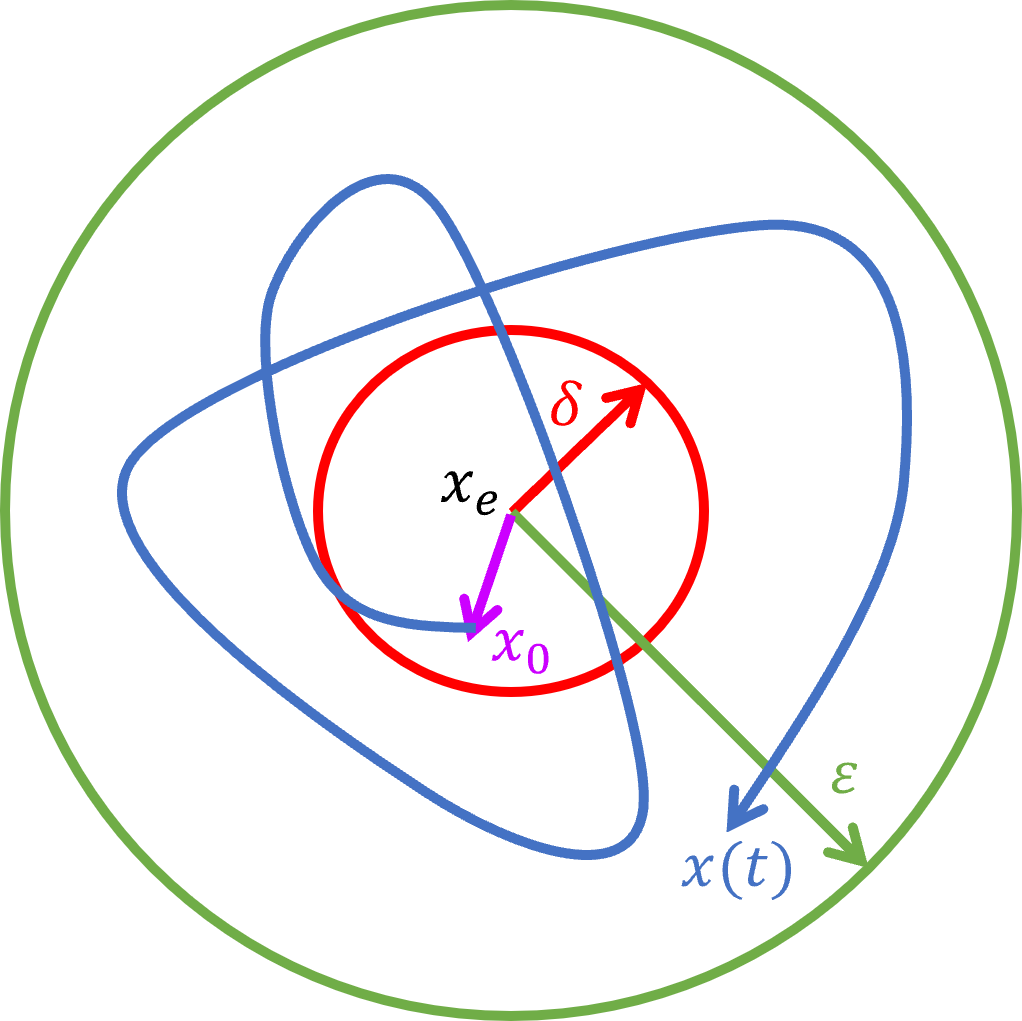
\includegraphics[scale=0.7]{Figuras/Lyapunov.png}
\end{figure}
* Mínima restricción que podemos imponer para satisfacer estabilidad.

\subsection{Definición Estabilidad Asintótica}
$x_e$ es asintóticamente estable si existe $\delta>0$ tal que:
\begin{itemize}
    \item $||x_0-x_e||<\delta$
    \item $x_e$ es estable en el sentido de Lyapunov
    \item $\lim_{t\to\infty}x(t)=x_e$
\end{itemize}
\begin{figure}[H]
\centering
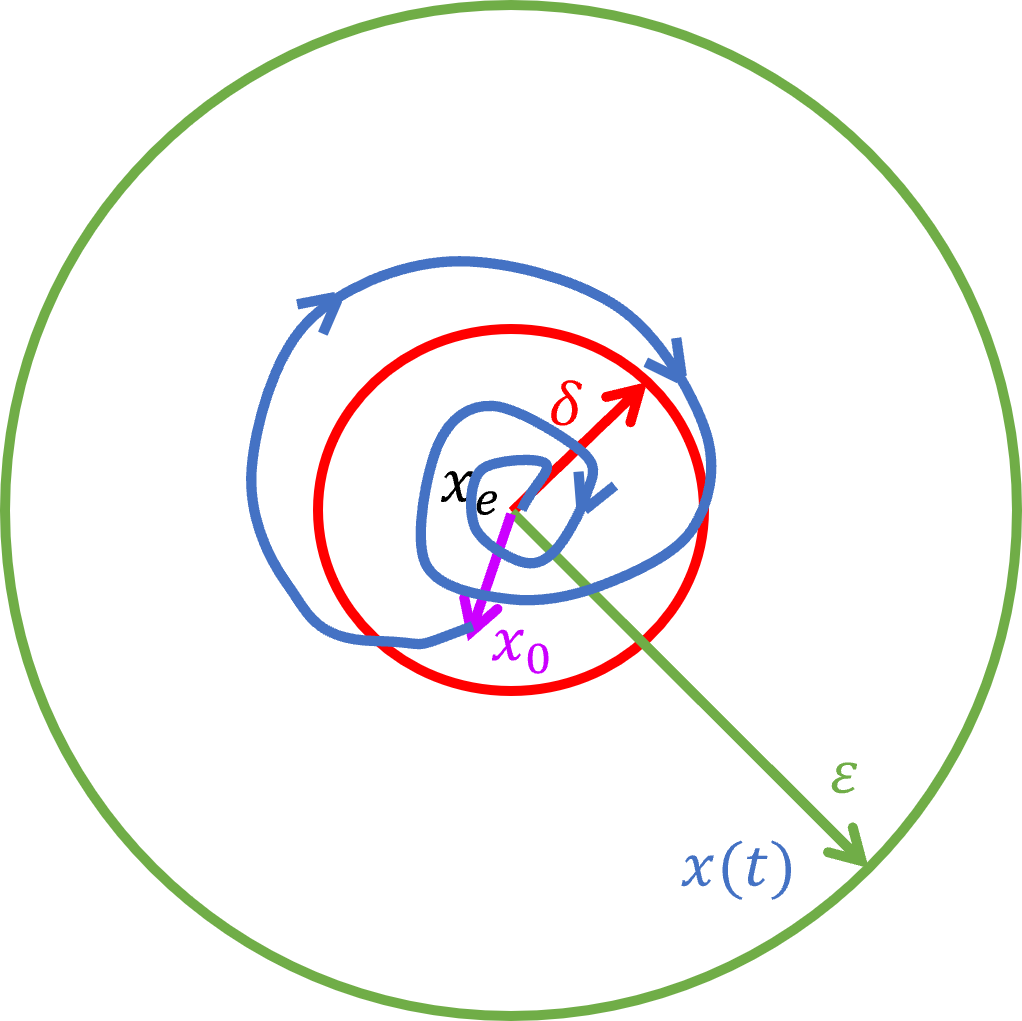
\includegraphics[scale=0.7]{Figuras/asintotica.png}
\end{figure}

\subsection{Definición Estabilidad Asintótica Global}
$x_e$ es estable asintótica global ssi es asintóticamente estable para $\delta \to \infty$.

\begin{table}[H]
    \centering
    \begin{tabular}{c|c|c|c|}
                & \raisebox{-\totalheight}{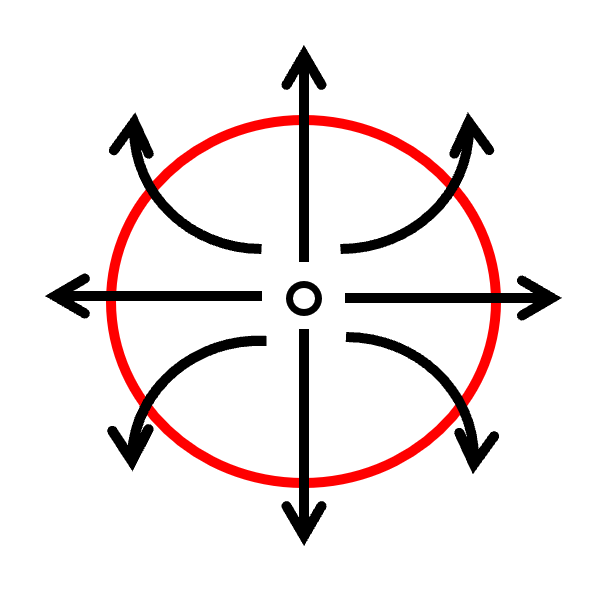
\includegraphics[scale=0.5]{Figuras/global1.png}} & \raisebox{-\totalheight}{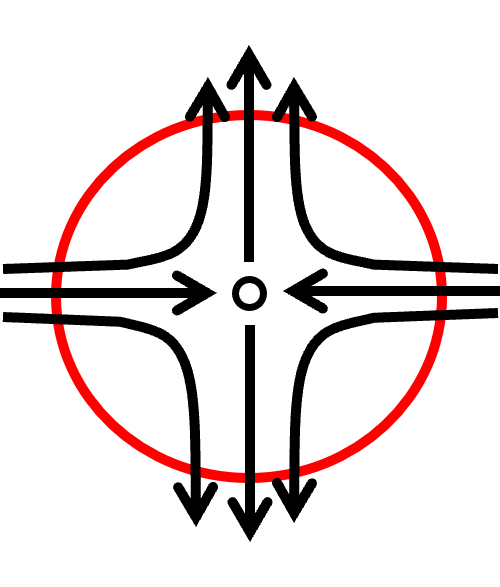
\includegraphics[scale=0.5]{Figuras/global2.png}} & \raisebox{-\totalheight}{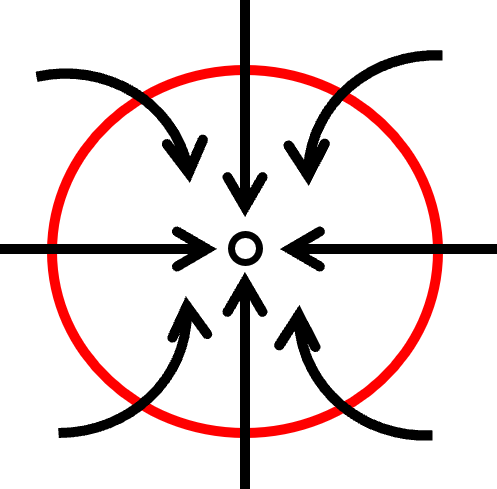
\includegraphics[scale=0.5]{Figuras/global3.png}}\\ \hline
         Estable & \xmark & \xmark & \cmark\\
         Asint. Est. & \xmark & \xmark &\cmark \\
         Goblal Asint. Est. & \xmark & \xmark & \textbf{???}
    \end{tabular}
\end{table}


\section{Límites de Estabilidad para sistemas LTI}
Sea $\dot{x}=Ax$, $x(t)\in \mathbb{R}^n$, $x(0)=x_0$.\\
Solución: $x(t)=\phi(t)x_0$, donde $\phi(t)=e^{At}$.\\
\par Suponiendo que $\phi(t)$ es finita,
$$||\phi(t)||=||e^{At}||\leq\beta<\infty $$
Luego:
\begin{align*}
    x(t)-x_e &= \phi(t)x_0-x_e\\
    &= \phi(t)x_0-\phi(t)x_e\\
    &= \phi(t)[x_0-x_e]
\end{align*}
\underline{Nota}: Si $x_0=x_e$, entonces $x(t)=x_e$ para $\phi(t)x_e=x_e$.\\
\par Entonces:
\begin{align*}
    ||x(t)-x_e||=||\phi(t)[x_0-x_e]||\leq||\phi(t)||\cdot||x_0-x_e||
\end{align*}
Si $||x_0-x_e||<\delta$ y $||x(t)-x_e||\leq \beta||x_0-x_e||$.\\
\par Sea $\varepsilon$, tal que $\delta=\varepsilon/\beta$.
$$\Longrightarrow ||x(t)-x_e||<\varepsilon $$
Por lo tanto, si $\phi(t)$ es finito, implica que $x_e$ es estable en el sentido de Lyapunov.\\
\par $\phi(t)$ es finito si y solo si $A$ es Hurwitz:
\begin{align*}
    \text{Re}\left(\text{eig}(A)\right)<0\Longrightarrow \text{Estabilidad}
\end{align*}

\section{Función Candidata de Lyapunov}
\underline{Definición}: Sea una función $V(x)$, $\mathbb{R}^n\to \mathbb{R}$, tal que: 
\begin{itemize}
    \item $V(x_e)=0$
    \item $V(x)>0$, $\forall x\neq x_e$ ($V$ es una función definida positiva)
    \item $V$ y su primera derivada son finitas
\end{itemize}
Entonces, $V$ es una función candidata de Lyapunov.\\
\par \underline{Teorema}: Si $V(x)$ s una función candidata de Lyapunov para $x_e$ en una región $\Omega$ vecina a $x_e$:
\begin{itemize}
    \item[a)] $x_e$ es estable en el sentido de Lyapunov si:
    $$\frac{dV}{dt}\leq 0, ~\forall x\in \Omega $$
    \item[b)] $x_e$ es asintóticamente estable si:
    $$\frac{dV}{dt}< 0, ~\forall x\in \Omega$$
    \item[c)] $x_e$ es global asintóticamente estable si:
    $$\frac{dV}{dt}< 0, ~\forall x\in \Omega$$
    donde $\Omega \in \mathbb{R}^n$ y $V$ no tiene límite radial.
\end{itemize}

\underline{Ilustración}: Sea $x=\begin{bmatrix}x_1\\ x_2\end{bmatrix}$, $x\in \mathbb{R}^2$, $x_e=0$.\\
Sea $V(x)=x^\top x$ es una función candidata de Lyapunov.

\begin{figure}[H]
\centering
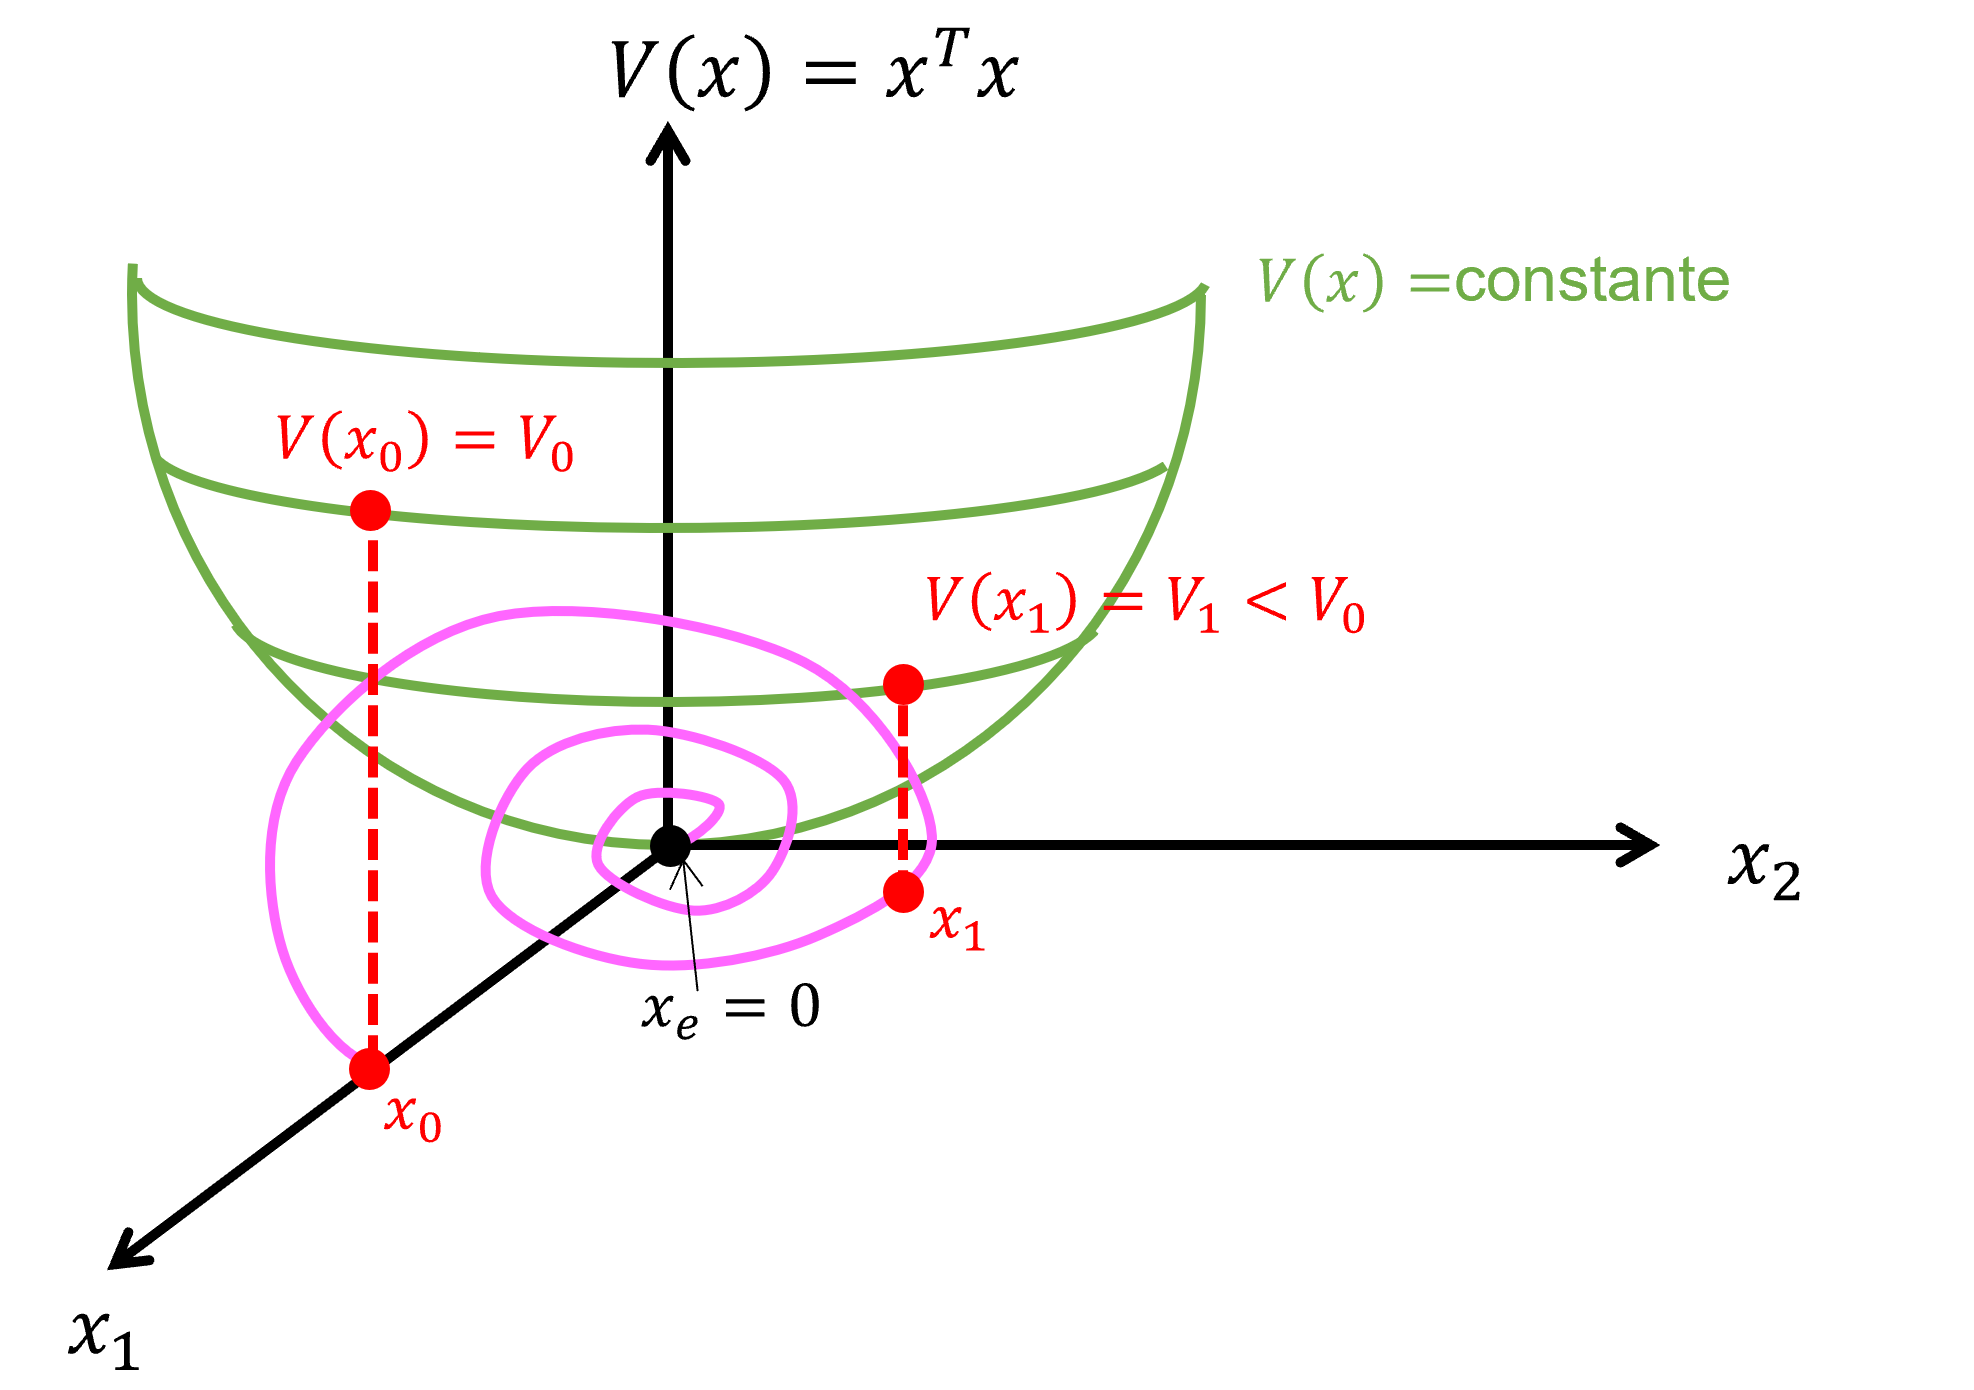
\includegraphics[scale=0.7]{Figuras/ilu_lyapunov.png}
\end{figure}



$$\frac{dV}{dt}<0 \Longrightarrow V(x) \quad V(x) \text{ decrece cuando t aumenta}$$

Notar que $V=V(x(t))$. Entonces:
\begin{align*}
    \frac{dV}{dt} &= \frac{\partial V}{\partial x}\cdot \frac{\partial x}{\partial t}  \quad \text{Regla de la cadena}\\
    &= \sum_{i=1}^n \frac{\partial V}{\partial x_i}\cdot\frac{\partial x_i}{\partial t}\\
    &= \begin{bmatrix}\frac{\partial V}{\partial x_1} &...& \frac{\partial V}{\partial x_n}\end{bmatrix}\begin{bmatrix}\dot{x}_1\\ \vdots \\ \dot{x}_n\end{bmatrix}\\
    &= \nabla V\cdot \dot{x}
\end{align*}

\begin{align*}
    \frac{dV}{dt}=\nabla V\cdot \dot{x}<0, ~\forall t
\end{align*}

\underline{Ilustración}: Dibujemos una línea de contorno de $V(x)$: \\
\begin{figure}[H]
\centering
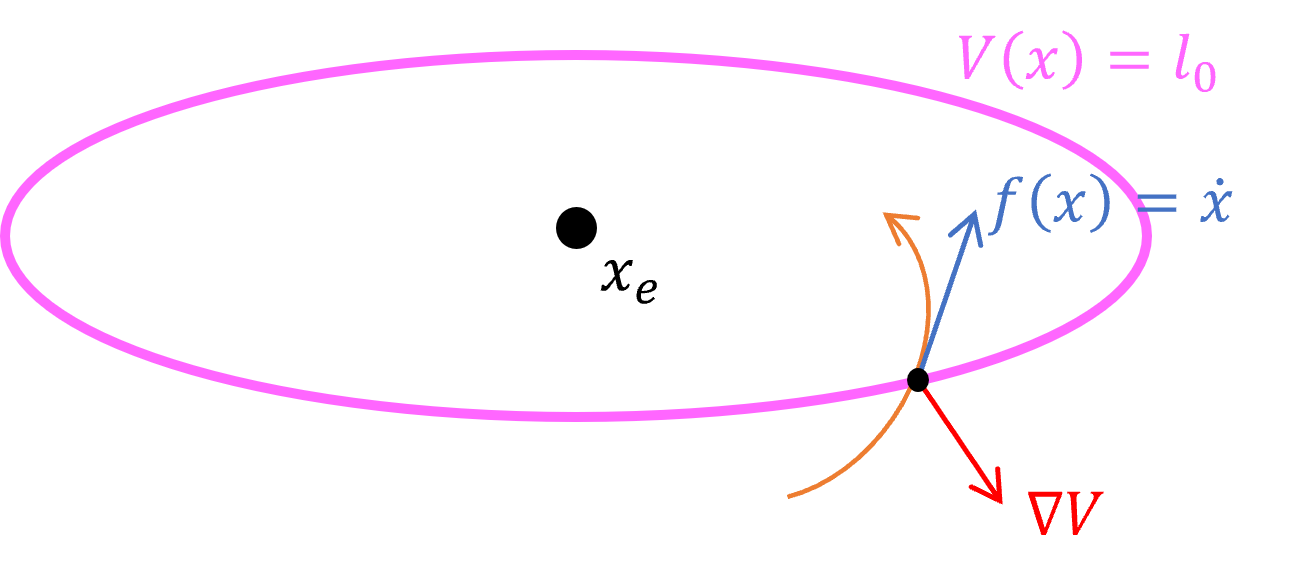
\includegraphics[scale=0.7]{Figuras/ilu_lyapunov2.png}
\end{figure}
$\nabla V\cdot f(x)<0 \Longrightarrow$ Entonces el sistema se acerca a $x_e$.\\
$\Longrightarrow x_e$ es un punto de atracción ``sumidero''.\\

\par Para $\dot{x}=Ax$, y sea $V(s)=x^\top Px$, donde $P$ es una matriz definida positiva y simétrica.
$$\frac{dV}{dt}=\nabla V\cdot \dot{x}<0 $$ para un sistema asintóticamente estable.\\
\begin{align*}
    \nabla V=\frac{\partial}{\partial \tend{x}} (\tend{x}^\top \tenq{P}\tend{x})=2\tenq{P}\tend{x} \quad \text{Por demostrar}
\end{align*}
Entonces:
\begin{align*}
    \frac{dV}{dt} &= (2Px)^\top (Ax)= (2x^\top P^\top)(Ax)\\
    &= (x^\top P^\top)(Ax)+x^\top P^\top Ax\\
    &= (Px)^\top(Ax)+x^\top PAx\\
    &= (Ax)^\top(Px)+x^\top PAx\\
    &= x^\top A^\top Px+x^\top PAx\\
    &= x^\top (A^\top P+PA)x<0
\end{align*}

Por lo tanto, $A^\top P+PA\prec 0$ definida negativa para que el sistema sea asintóticamente estable.\\
\par Sea $Q$ una matriz definida positiva y simétrica, tal que:
\begin{align*}
    A^\top P+PA &= -Q\\
    A^\top P+PA+Q &= \emptyset \quad \text{Ecuación de Lyapunov}
\end{align*}

\underline{Teorema}: Dado $Q \succ 0$, existe un $P\succ 0$ simétrica que satisface:
$$A^\top P+PA+Q=\emptyset $$
entonces, $\dot{x}=Ax$ es asintóticamente estable.



\section{Teorema de Cayley-Hamilton}
\underline{Teorema}: Sea una matriz $A\in\mathbb{R}^{n\times n}$, cuya ecuación característica está dada por el siguiente polinomio de orden n:
\begin{align*}
    \Delta (A)=\text{det}(sI-A)=s^n+\alpha_{n-1}s^{n-1}+...+\alpha_1s+\alpha_0=0
\end{align*}
donde $\alpha_i\in\mathbb{R}$, $i\in [0,n-1]$, son los coeficientes del polinomio característico de $A$. \\
\par Entonces, la matriz $A$ también satisface la ecuación característica:
\begin{align*}
    \Delta (\tenq{A})=\tenq{A}^n+\alpha_{n-1}\tenq{A}^{n-1}+...+\alpha_1\tenq{A}+\alpha_0\tenq{I}=\tenq{0}
\end{align*}

Del teorema, podemos despejar $\tenq{A}^n$:
\begin{align*}
    \tenq{A}^n &= -\left[\tenq{A}^n+\alpha_{n-1}\tenq{A}^{n-1}+...+\alpha_1\tenq{A}+\alpha_0\tenq{I} \right]
\end{align*}

El poder de una matriz se escribe como una serie polinomial de orden igual al exponente del poder.\\
\par $\Longrightarrow$ Este resultado es útil para evaluar la matriz de transición $\phi(t)$
\begin{align*}
    \phi(t)=e^{At}=\sum_{i=0}^\infty \beta_i(t)A^i \overset{\text{(C-H)}}{=} \sum_{i=0}^{n-1}\gamma_i(t)A^i
\end{align*}
\underline{Nota}: Este resultado es útil para evaluar $\phi(t)$ como una serie finita en términos de $A^i$.

\section{Controlabilidad}
La controlabilidad es una propiedad d cualquier sistema dinámico.\\
\par $\Longrightarrow$ Sea el sistema LTI: $\dot{x}=Ax+Bu$, $x\in \mathbb{R}^n$, $u\in\mathbb{R}^p$. Buscamos $u(t)$ tal que los estados vayan de $x(t)$ a cero en un tiempo finito $t_1$. \\
\par \underline{Solución}: $x(t)=\phi(t)x_0+\int_0^t \phi(t-\tau)Bu(\tau)d\tau$
\begin{align*}
    x(t_1)=0=\phi(t_1)x_0+\int_0^{t_1} \phi(t_1-\tau)Bu(\tau)d\tau
\end{align*}

\underline{Aparte}: $\phi(t_1-\tau)=e^({A(t_1-\tau)}=e^A\cdot e^{-A\tau}=\phi(t_1)\phi(-\tau)$

\begin{align*}
    \Longrightarrow 0 &=\phi(t_1)\left[x_0+\int_0^{t_1}\phi(-\tau)Bu(\tau)d\tau\right] \\
    -x_0 &= \int_0^{t_1}\phi(-\tau)Bu(\tau)d\tau
\end{align*}

Por el teorema de Cayley-Hamilton:
\begin{align*}
    \phi(-\tau)=m_0(\tau)I+m_1(\tau)A+m_2(\tau)A^2+...+m_{n-1}(\tau)A^{n-1}
\end{align*}

Entonces:
\begin{align*}
    -x_0 &= \int_0^{t_1}\left[m_0(\tau)BI+m_1(\tau)AB+m_2(\tau)A^2B+...+m_{n-1}(\tau)A^{n-1}B \right]u(\tau)d\tau\\
    \Longrightarrow -x_0 &= \int_0^{t_1} \sum_{j=0}^{n-1}A^jBm_j(\tau)u(\tau)d(\tau)\\
    \Longrightarrow -x_0 &= \sum_{j=0}^{n-1}A^jB \int_0^{t_1} m_j(\tau)u(\tau)d\tau
\end{align*}

Cada término de la integral es nu vector constante de dimensión $p\times 1$
\begin{align*}
    \Longrightarrow v_j = \int_0^{t_1}m_j(\tau)u(\tau)d\tau
\end{align*}

\begin{align*}
    \Longrightarrow -x_0 &= \sum_{j=0}^{n-1}A^jBv_j =Bv_0+ABv_1+...+A^{n-1}Bv_{n-1}\\
     \Longrightarrow -x_0 &= \left[
    \begin{array}{c|c|c|c|c}
     B & AB & A^2B & ... & A^{n-1}B
    \end{array}\right] \left[
    \begin{array}{c}
     v_0\\ \hline v_1 \\ \hline v_2 \\ \hline \vdots \\ \hline v_{n-1} 
    \end{array}\right]
\end{align*}
Se define:
\begin{align*}
    \mathcal{C}=\left[
    \begin{array}{c|c|c|c|c}
     B & AB & A^2B & ... & A^{n-1}B
    \end{array}\right] \quad \text{Matriz de controlabilidad}
\end{align*}
Este resultado indica que cualquier vector $-x_0$ puede ser expresado como una combinación lineal de las columnas de la matriz $\mathcal{C}$. Esta matriz $mathcal{C}$ debe tner rango igual a $n$para escribir $-x_0\in \mathbb{R}^n$.\\
\par Por lo tanto, un sistema LTI, $\dot{x}=Ax_Bu$, $A\in \mathbb{R}^{n\times n}$, $B\in \mathbb{R}^{n\times p}$, es controlable si y solo si:
\begin{align*}
    \text{rank}(\mathcal{C})=n
\end{align*}

\underline{Nota}: Si $\text{rank}(\mathcal{C})<n$, entonces el sistema tiene no más de $n_e$ estados controlables.\\
\par \underline{Definición}: Si el sistema tiene estados inestables, pero controlables, entonces se dice que estos estados son \textcolor{red}{estabilizables}. Por lo tanto, puede diseñar $u(t)$ tal que el sistema cerrado tenga todos sus estados estables.\\
\par Sea el sistema LTI, $\dot{x}=Ax+Bu$, y sea $T$ una matriz de transformación tal que $x=Tz$, donde $\dot{z}=A_cz+B_cu$, es una realización CCF.\\
\par \underline{Entonces, el sistema es controlable ssi $T$ existe.}

\section{Observabilidad}
Asuma el sistema autónomo LTI:
\begin{align*}
    \dot{x} &= Ax, \quad x\in\mathbb{R}^n\\
    y &= Cx, \quad y\in\mathbb{R}^r
\end{align*}

\begin{align*}
    \begin{array} {|c|}
  \hline \text{Caja}\\ 
  \text{Negra} \\
  \hline 
\end{array} \longrightarrow y\in\mathbb{R}^r
\end{align*}

Sabemos que la solución $x(t)$: 
\begin{align*}
    x(t)=\phi(t)x_0\Longrightarrowy(t)=Cx(t)=C\phi(t)x_0
\end{align*}
Además: $y(t0=Ce^{At}x_0$
\begin{align*}
    y(t) &= C\left[l_0(t)I+l_1(t)A+l_2(t)A^2+...+l_{n-1}(t)A^{n-1} \right]x_0\\
    y(t) &= \left[
    \begin{array}{c|c|c|c|c}
     l_0(t) & l_1(t) & l_2(t) & ... & l_{n-1}(t)
    \end{array}\right] \left[
    \begin{array}{c}
     C\\ \hline CA \\ \hline CA^2 \\ \hline \vdots \\ \hline CA^{n-1} 
    \end{array}\right]
\end{align*}

Se define:
\begin{align*}
    \mathcal{O}=\left[
    \begin{array}{c}
     C\\ \hline CA \\ \hline CA^2 \\ \hline \vdots \\ \hline CA^{n-1} 
    \end{array}\right] \quad \text{Matriz de observabilidad}
\end{align*}

Si $\mathcal{O}$ no es de rango completo, entonces podemos elegir $x_0\neq 0$ tal que $y(0)=0$, porque $t_0$ puede producir el mismo resultado. \\
\par \underline{Por lo tanto, un sistema LTI es observable ssi $\text{rank}(\mathcal{O})=n$}\\
\par \underline{Definición}: Si un estado es inestable, pero observable, entonces dicho estado se dice que es \textcolor{red}{detectable}. 


\section{Observadores}
Suponga un sistema dinámico:
\begin{align*}
    \dot{x} &= f(x,u)\\
    y &= g(x,u)
\end{align*}
Ejemplo: 
\begin{figure}[H]
\centering
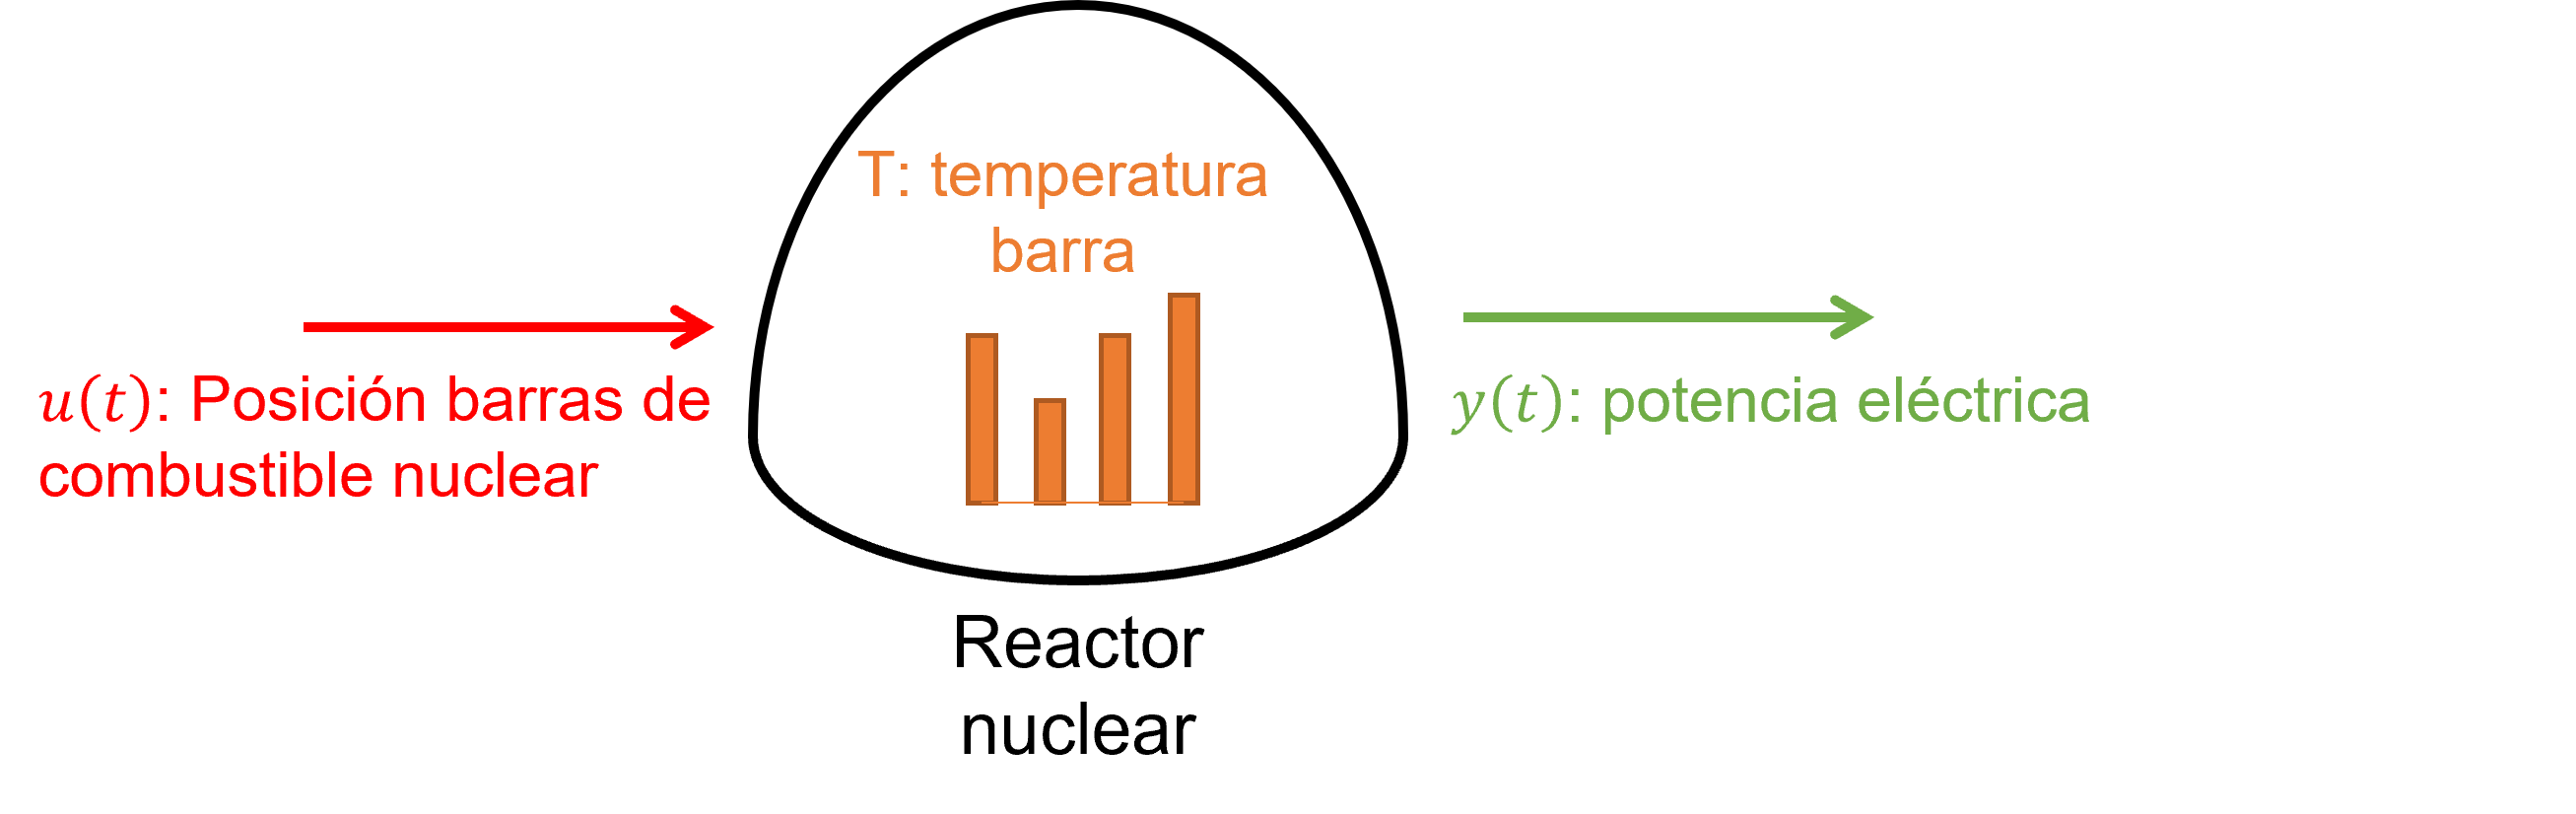
\includegraphics[scale=0.7]{Figuras/nuclear.png}
\end{figure}

¿Es posible determinar los estados internos del sistema, utilizando solo las señales de entrada y salida $\{u(t), y(t)\}$?\\
\par \underline{Respuesta}: Sí, pero con la condición que el sistema sea \textcolor{red}{observable}.\\
\par \underline{Notación}: 
\begin{itemize}
    \item $x(t)$: estados del sistema
    \item $\hat{x}(t)$: estados estimados
    \item $\tilde{x}(t)=x(t)-\hat{x}(t)$: error de estimación
\end{itemize}

\underline{Objetivo}: Diseñar un estimador/observador para $x(t)$.\\
\par Sea un sistema LTI:
\begin{align*}
    \dot{x} &= Ax+Bu\\
    y &= Cx
\end{align*}
con condición inicial $x(0)=x_0$. \\
\par Estimador: $\dot{\hat{x}}=A\hat{x}+Bu$, $\hat{x}(0)=?$ (cualquier número).\\
\par Revisemos la dinámica del error del estimador:

\begin{align*}
    \dot{\tilde{x}} &= \frac{d}{dt}(x-\hat{x})=\dot{x}-\dot{\hat{x}}\\
    &= (Ax+Bu)-(A\hat{x}+Bu)=A(x-\hat{x})
\end{align*}
Por lo tanto, $\dot{\hat{x}}=A\tilde{x}$: error del estimador posee la misma dinámica del sistema LTI.\\
\par \underline{Estrategia}: Si mis estados decaen a cero, entonces voy a diseñar un estimador tal que el error de la estimación decae con la misma tasa que el sistema.
\begin{figure}[H]
\centering
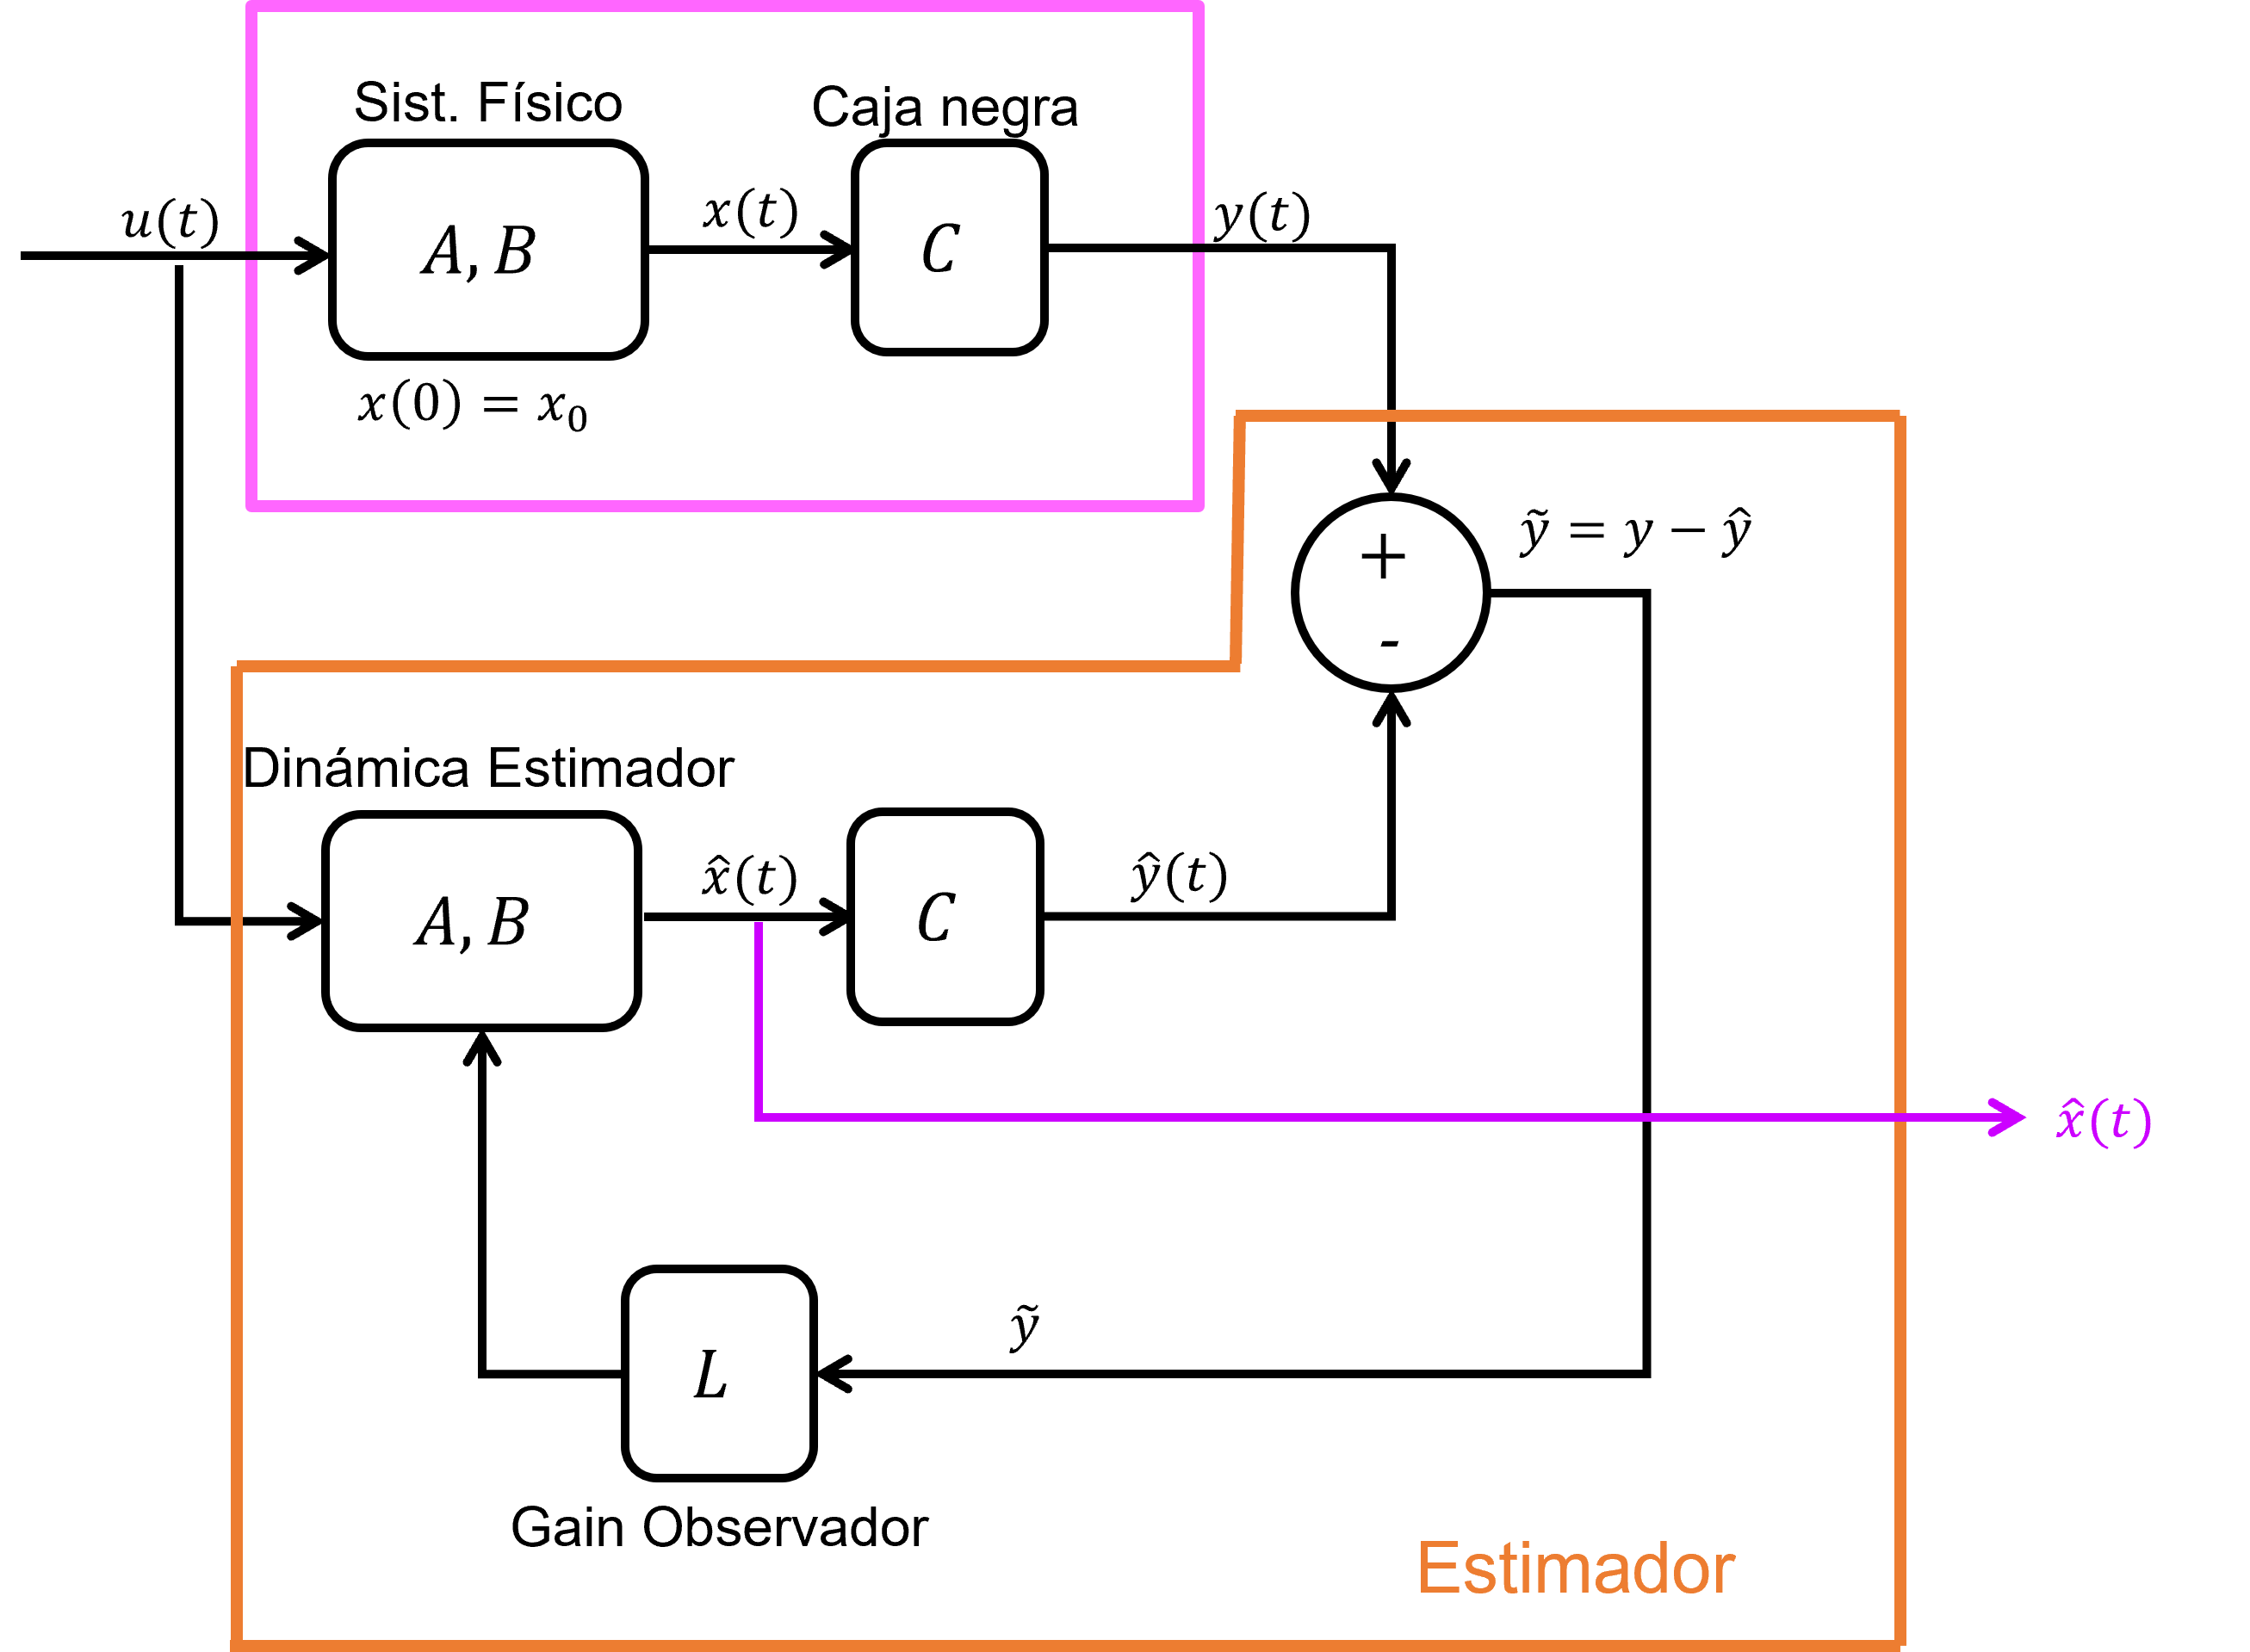
\includegraphics[scale=0.7]{Figuras/observador.png}
\end{figure}
\begin{figure}[H]
\centering
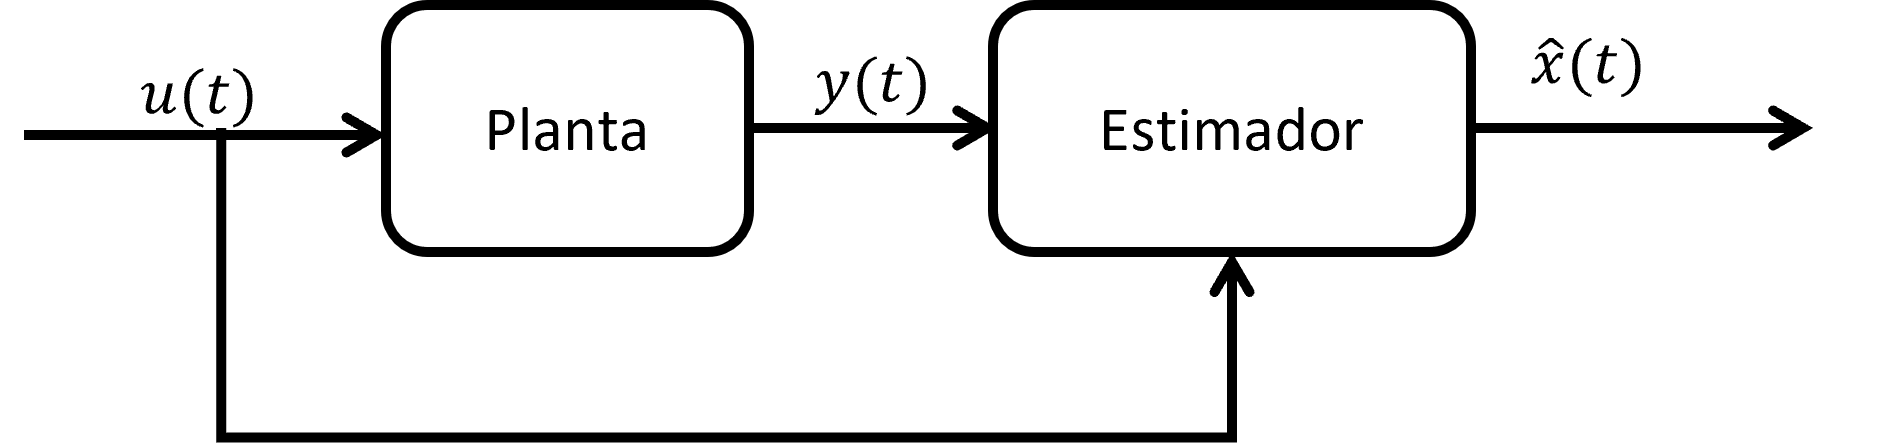
\includegraphics[scale=0.7]{Figuras/observador2.png}
\end{figure}

\section{Diseño de Observador de Estados}
\begin{align*}
    \dot{\hat{x}}=A\hat{x}+Bu+L\tilde{y}
\end{align*}
Sea 
\begin{align*}
    L=\left[
    \begin{array}{c}
     l_1 \\ l_2\\ \vdots\\ l_n 
    \end{array}\right], \quad L \in \mathbb{R}^{n\times r}, \quad x,y \in \mathbb{R}^n 
\end{align*}

Ecuación de error de estado:
\begin{align*}
    \dot{\tilde{x}}=\dot{x}-\dot{\hat{x}} &= (Ax+Bu)-(A\hat{x}+Bu+L\tilde{y})\\
    &= A\tilde{x}-L(y-\hat{y})\\
    &= A\tilde{x}-L(Cx-C\hat{x})\\
    &= A\tilde{x}-LC\tilde{x}\\
    \dot{\tilde{x}} &= (A-LC)\tilde{x}
\end{align*}
Notar que para que $(A-LC)$ cumpla estabilidad, los polos deben estar al lado izquierdo del plano complejo.\\
\par $\Longrightarrow$ Vamos a diseñar $L$, ubicando apropiadamente los polos del sistema cerrado $(A-LC)$ $\Longrightarrow$ \textcolor{red}{POLE PLACEMENT}.\\
\par \underline{Caso particular}: $x\in\mathbb{R}^n$, $u\in\mathbb{R}$, $y\in\mathbb{R}$.\\
\par Forma Canónica Observable. 
\par Recordar: 
\begin{align*}
    G(s) = \frac{b_0}{s^n+a_{n-1}s^{n-1}+...+a_1s+a_0}
\end{align*}

\begin{align*}
\tenq{A_o}=\left[
    \begin{array}{c|cccc}
     -a_{n-1} & 1 & & & 0 \\ 
     -a_{n-2} & & 1 & & \\
     \vdots   & & & \ddots & \\
     -a_1     & 0 & & & 1 \\ \hline
     -a_0     & 0 & 0 & \dots & 0   
    \end{array}\right], \quad \tenq{A_o}\in \mathbb{R}^{n\times n}
\end{align*}
\begin{align*}
\tenq{B_o}=\left[
    \begin{array}{c}
     b_{n-1} \\
     b_{n-2}\\
    \vdots\\
     b_1 \\ \hline
     b_0
    \end{array}\right], \quad \tenq{B_o}\in \mathbb{R}^{n\times 1}
\end{align*}
\begin{align*}
\tenq{C_o}=\left[
    \begin{array}{c|ccc}
     1 & 0 & \dots & 0
    \end{array}\right], \quad \tenq{C}_o\in \mathbb{R}^{1\times n}
\end{align*}
Si $y\in\mathbb{R}$, entonces:
\begin{align*}
    L=\left[
    \begin{array}{c}
     l_{n-1} \\ l_{n-2}\\ \vdots\\ l_0 
    \end{array}\right] 
\end{align*}
\underline{Objetivo}: Determinar los $l_i$, $i\in[0,n-1]$
\begin{align*}
    LC_o&=\left[
    \begin{array}{c}
     l_{n-1} \\ l_{n-2}\\ \vdots\\ l_0 
    \end{array}\right] \left[
    \begin{array}{c c c c}
     1 & 0 & ... & 0
    \end{array}\right] =\left[
    \begin{array}{c|c}
     l_{n-1} & \\ \vdots & \tenq{0} \\ l_0 & 
    \end{array}\right] \\
    A_o-LC_o &= \left[ \begin{array}{c|c c c}
     -a_{n-1}-l_{n-1} & & & \\  -a_{n-2}-l_{n-2} & & & \\ \vdots & & \tenq{I} & \\-a_1-l_1 & & & \\ \hline \\ -a_0-l_0 & 0 & ... & 0
    \end{array}\right] 
\end{align*}
Ecuación característica: 
\begin{align*}
    \Delta(A_o-LC_o) =s^n+(a_{n-1}+l_{n-1})s^{n-1}+...+(a_1+l_1)s+(a_0+l_0)=0    
\end{align*}
donde $\lambda_i=(a_i+l_i)$, $i\in[0,n-1]$, son los coeficientes del polinomio característico, asociado a la ubicación de polos deseada:
\begin{align*}
    \prod_{i=0}^{n-1}(s-p_i)=s^n+\lambda_{n-1}s^{n-1}+...+\lambda_1s+\lambda_0=0
\end{align*}
donde $p_i$ es la posición de los polos deseada.\\
\par Finalmente:
\begin{align*}
    l_i=a_i-\lambda_i,\quad i\in[0,n-1]
\end{align*}
\par \underline{Nota}: en Matlab, utilizar el comando \texttt{place()}. \\
\par \underline{Nota}: Si el sistema no está escrito en OCF, entonces se puede realizar una transformación de similitud con matriz T. Esta matriz T existe ssi el sistema es observable.

\section{Principio de Separación}
Estudiemos el siguiente sistema LTI cerrado:
\begin{figure}[H]
\centering
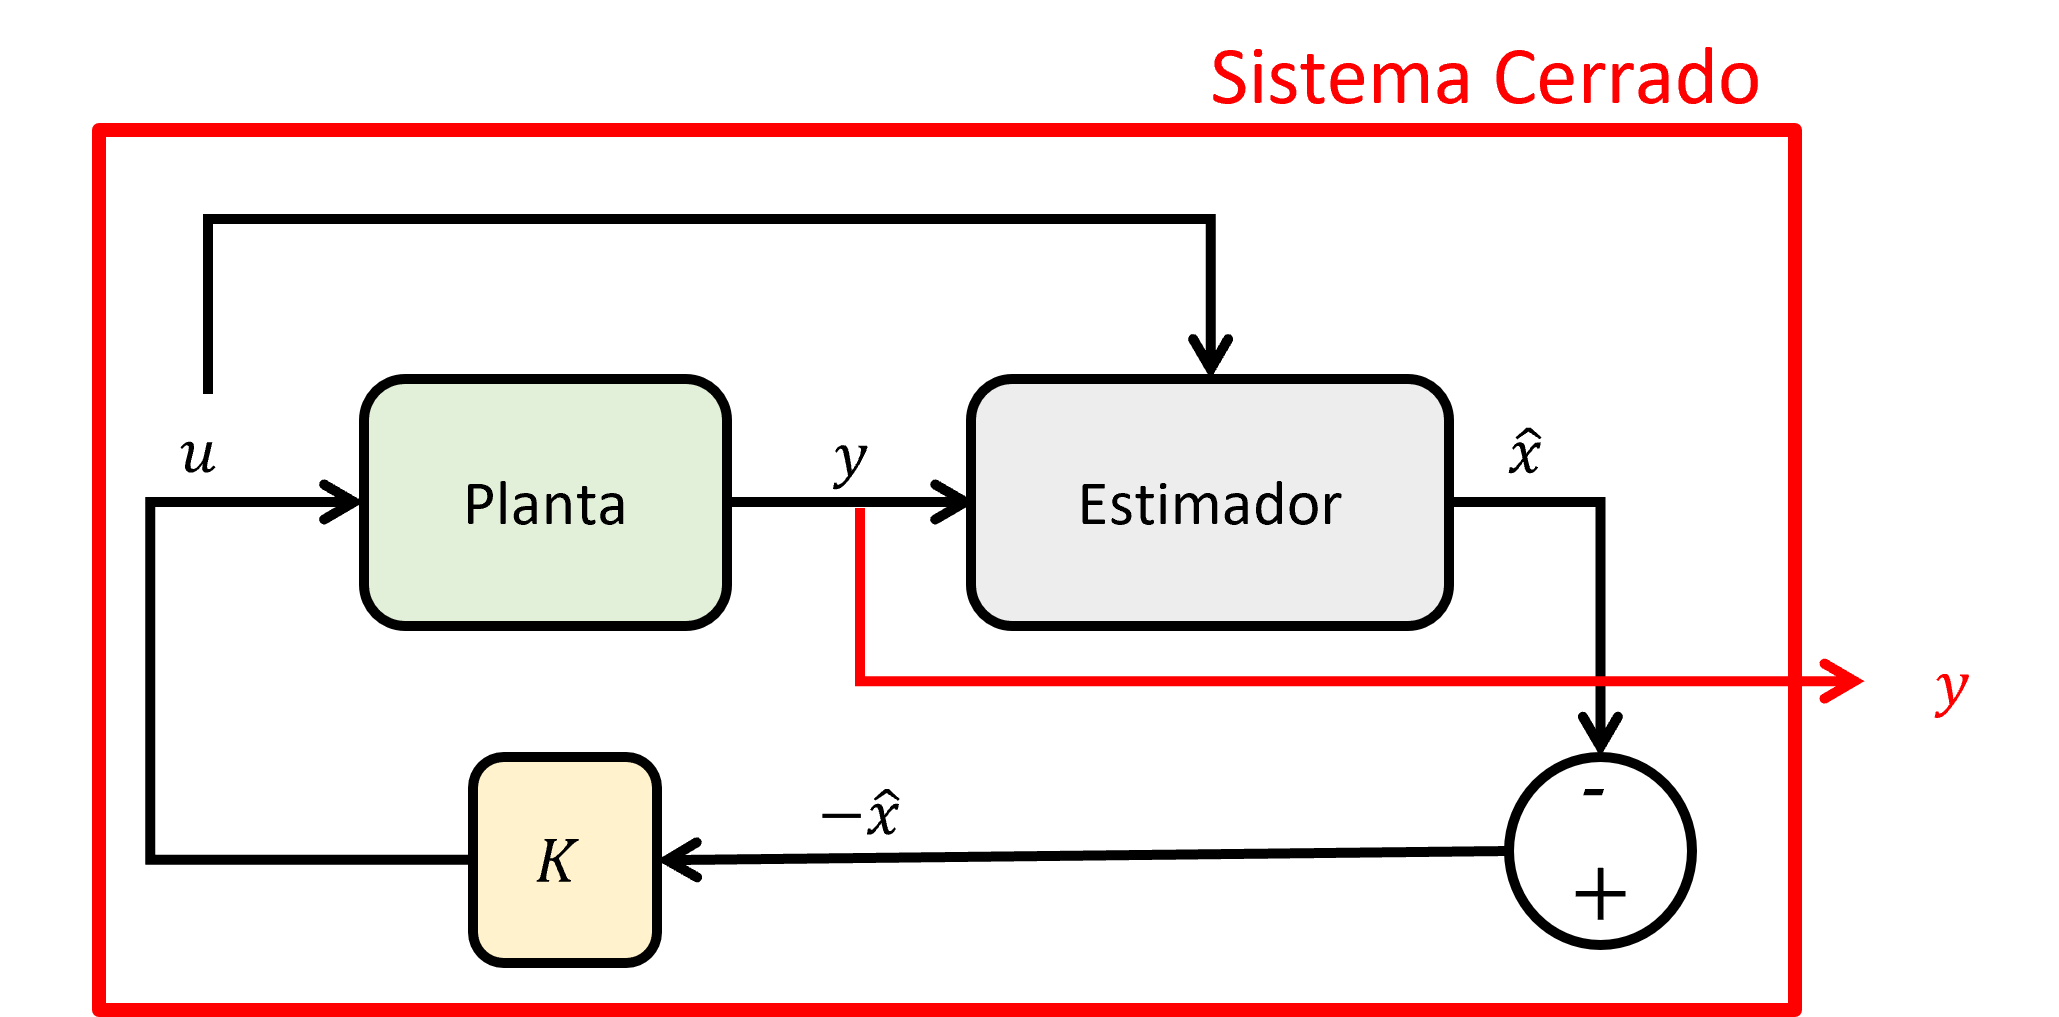
\includegraphics[scale=0.7]{Figuras/ppio_separacion.png}
\end{figure}

\setcounter{equation}{0}
\begin{subequations}
\begin{align}
    \text{Planta: }  \dot{x} &= Ax+Bu\\
    y &= Cx
    \end{align}
\end{subequations}
\begin{subequations}
    \begin{align}
    \text{Controlador: }  u &= -k\hat{x}
    \end{align}
\end{subequations} 
\begin{subequations}
    \begin{align}
    \text{Estimador: }  \dot{\hat{x}}&= A\hat{x}+Bu+L\tilde{y}\\
     \hat{y} &= C\hat{x}\\
     \tilde{x} &= x-\hat{x}\\
    \tilde{y} &= y-\hat{y}
\end{align}
\end{subequations}

Vamos a obtener una expresión para el sistema cerrado:
\begin{align}
    \text{(3.2a) y (3.3c):} \quad u&=-K(c-\tilde{x})\\
    \text{(3.4) y (3.1a):} \quad \dot{x} &= Ax-BK(x\tilde{x})\\
    \Longrightarrow \dot{x} &= (A-BK)x+BK\tilde{x}\\
    \text{(3.3c) y (3.3a):} \quad \tilde{x} &= x-\hat{x}\\
    \dot{\tilde{x}} &= \dot{x}-\dot{\hat{x}}\\
    \Longrightarrow \dot{\tilde{x}} &= (Ax+Bu)-(A\hat{x}+Bu+L\tilde{y})\\
    \Longrightarrow \dot{\tilde{x}} &= A\tilde{x}-LC \tilde{x}\\
    \Longrightarrow \dot{\tilde{x}} &= (A-LC)\tilde{x}
\end{align}
Definir $z=\left[
    \begin{array}{c}
     x \\ \tilde{x} 
    \end{array}\right]$, estados del sistema cerrado.\\
\par Ecuación de estado del sistema cerrado:
\begin{align*}
    \dot{z}=\left[
    \begin{array}{c}
     \dot{x} \\ \dot{\tilde{x}} 
    \end{array}\right] = \left[
    \begin{array}{cc}
     A-BK & BK \\ 0 & A-LC 
    \end{array}\right]\left[
    \begin{array}{c}
     x \\ \tilde{x} 
    \end{array}\right]
\end{align*}
Definimos:
\begin{align*}
    A_{CL} &= \left[
    \begin{array}{cc}
     A-BK & BK \\ 0 & A-LC 
    \end{array}\right]\\
    \Longrightarrow \dot{z}&=A_{CL}z
\end{align*}

Los polos de $A_{CL}$ se obtienen al resolver la ecuación característica:
\begin{align*}
    \text{det}(sI-A_{CL})&=0\\
    \Longrightarrow \text{det}(sI-(A-BK))\cdot\text{det}(sI-(A-LC)) &=0
\end{align*}
\begin{itemize}
    \item $\text{det}(sI-(A-BK))$: polos del subsistema planta + controlador
    \item $\text{det}(sI-(A-LC))$: polos del subsistema planta + observador 
\end{itemize}

Este resultado se conoce como el \textcolor{red}{principio de separación}.\\
\par Diseñar $K$ y $L$ por separado, luego agrupar y construir el sistema de control cerrado.


